\def\advent@xxiii@i{
  Each interior angle of a regular triangle is $60^\circ$.

  Each interior angle of a different regular polygon is $178^\circ$.
  How many sides does this polygon have?
}

\def\advent@xxiii@ii{
  Holly adds up the first six even numbers, then adds on half of the next even number.
  Her total is $49$.

  Next, Holly adds up the first $n$ even numbers then adds on half of the next even number.
  This time, her total is $465124$.
  What is $n$?
}

\def\advent@xxiii@iii{
  $190$ is the smallest multiple of $10$ whose digits add up to $10$.

  What is the smallest multiple of $15$ whose digits add up to $15$?
}

\def\advent@xxiii@iv{
  If $n$ is $1$, $2$, $4$, or $6$ then $(n! - 3)/(n - 3)$ is an integer.
  The largest of these numbers is $6$.

  What is the largest possible value of $n$ for which $(n! - 123)/(n - 123)$ is an integer?
}

\def\advent@xxiii@v{
  Put the digits $1$ to $9$ (using each digit exactly once) in the boxes so that the sums are correct.
  The sums should be read left to right and top to bottom ignoring the usual order of operations.
  For example, $4 + 3  \times 2$ is $14$, not $10$.
  Today's number is the product of the numbers in the red boxes.

  \grid@advent@xxiii@v{}{}{}{}{}{}{}{}{}
}

\def\crscale{1.5}
\definecolor{cry}{rgb}{1,1,0.663}
\definecolor{crb}{rgb}{0.667,1,1}
\definecolor{crg}{rgb}{0.671,1,0.663}
\definecolor{crp}{rgb}{1,0.667,1}
\newcommand\crvert[3]{\filldraw[ultra thick,fill=#1] (#2,#3) rectangle (#2+1,#3-2);}
\newcommand\crhorz[3]{\filldraw[ultra thick,fill=#1] (#2,#3) rectangle (#2+2,#3-1);}
\def\advent@xxiii@vi{
  There are $5$ ways to tile a $4 \times 2$ rectangle with $2 \times 1$ pieces:

  \begin{center}
    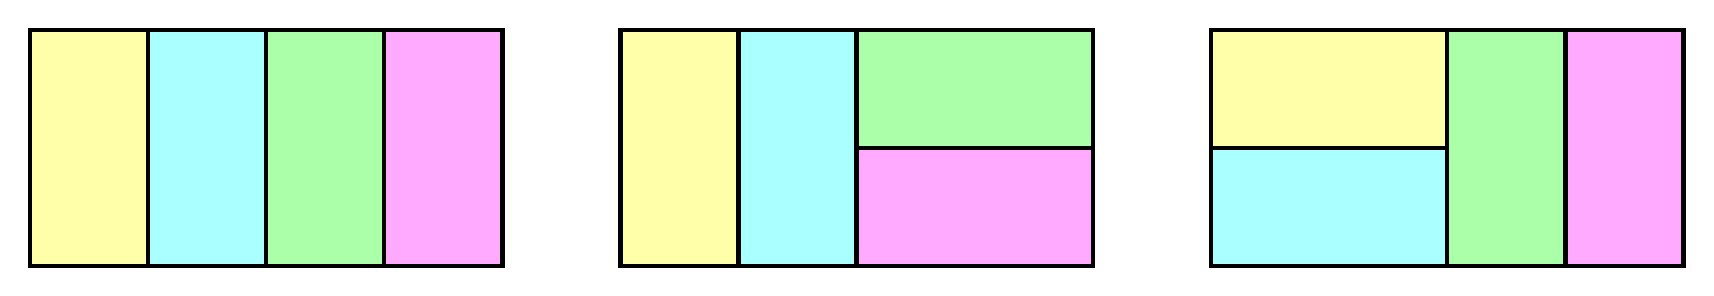
\begin{tikzpicture}[scale=\crscale]
      \crvert{cry}{0}{0}
      \crvert{crb}{1}{0}
      \crvert{crg}{2}{0}
      \crvert{crp}{3}{0}

      \crvert{cry}{5}{0}
      \crvert{crb}{6}{0}
      \crhorz{crg}{7}{0}
      \crhorz{crp}{7}{-1}

      \crhorz{cry}{10}{0}
      \crhorz{crb}{10}{-1}
      \crvert{crg}{12}{0}
      \crvert{crp}{13}{0}
    \end{tikzpicture}

    \vspace{0.3cm}

    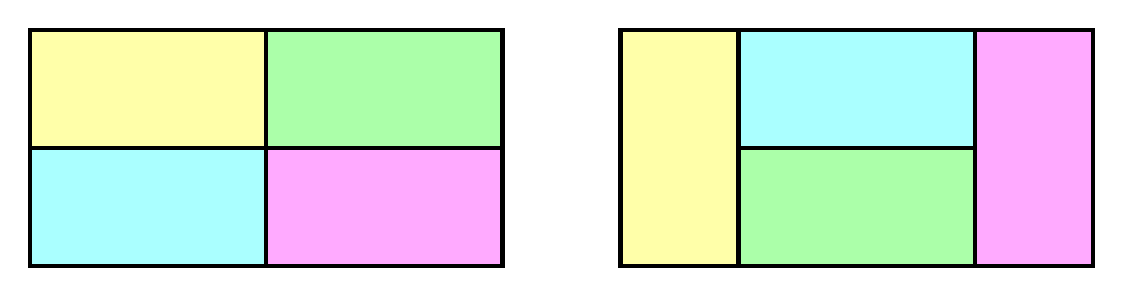
\begin{tikzpicture}[scale=\crscale]
      \crhorz{cry}{0}{0}
      \crhorz{crb}{0}{-1}
      \crhorz{crg}{2}{0}
      \crhorz{crp}{2}{-1}

      \crvert{cry}{5}{0}
      \crhorz{crb}{6}{0}
      \crhorz{crg}{6}{-1}
      \crvert{crp}{8}{0}
    \end{tikzpicture}
  \end{center}

  How many ways are there to tile a $12 \times 2$ rectangle with $2 \times 1$ pieces?
}